%%%%%%%%%%%%%%%%%%%%%%%%%%%%%%%%%%%%%%%%%
% Journal Article
% LaTeX Template
% Version 1.3 (9/9/13)
%
% This template has been downloaded from:
% http://www.LaTeXTemplates.com
%
% Original author:
% Frits Wenneker (http://www.howtotex.com)
%
% License:
% CC BY-NC-SA 3.0 (http://creativecommons.org/licenses/by-nc-sa/3.0/)
%
%%%%%%%%%%%%%%%%%%%%%%%%%%%%%%%%%%%%%%%%%

%----------------------------------------------------------------------------------------
%	PACKAGES AND OTHER DOCUMENT CONFIGURATIONS
%----------------------------------------------------------------------------------------

\documentclass[twoside]{article}

\usepackage{lipsum} % Package to generate dummy text throughout this template

\usepackage[sc]{mathpazo} % Use the Palatino font
\usepackage[T1]{fontenc} % Use 8-bit encoding that has 256 glyphs
\linespread{1.05} % Line spacing - Palatino needs more space between lines
\usepackage{microtype} % Slightly tweak font spacing for aesthetics
\usepackage{amsmath}

\usepackage[hmarginratio=1:1,top=32mm,columnsep=20pt]{geometry} % Document margins
\usepackage{multicol} % Used for the two-column layout of the document
\usepackage[hang, small,labelfont=bf,up,textfont=it,up]{caption} % Custom captions under/above floats in tables or figures
\usepackage{booktabs} % Horizontal rules in tables
\usepackage{float} % Required for tables and figures in the multi-column environment - they need to be placed in specific locations with the [H] (e.g. \begin{table}[H])
\usepackage{hyperref} % For hyperlinks in the PDF

\usepackage{lettrine} % The lettrine is the first enlarged letter at the beginning of the text
\usepackage{paralist} % Used for the compactitem environment which makes bullet points with less space between them
\usepackage{graphicx}
\usepackage{abstract} % Allows abstract customization
\renewcommand{\abstractnamefont}{\normalfont\bfseries} % Set the "Abstract" text to bold
\renewcommand{\abstracttextfont}{\normalfont\small\itshape} % Set the abstract itself to small italic text

\usepackage{titlesec} % Allows customization of titles
\renewcommand\thesection{\Roman{section}} % Roman numerals for the sections
\renewcommand\thesubsection{\Roman{subsection}} % Roman numerals for subsections
\titleformat{\section}[block]{\large\scshape\centering}{\thesection.}{1em}{} % Change the look of the section titles
\titleformat{\subsection}[block]{}{\thesubsection.}{1em}{} % Change the look of the section titles

\usepackage{fancyhdr} % Headers and footers
\pagestyle{fancy} % All pages have headers and footers
\fancyhead{} % Blank out the default header
\fancyfoot{} % Blank out the default footer
%\fancyhead[C]{Running title $\bullet$ November 2012 $\bullet$ Vol. XXI, No. 1} % Custom header text
\fancyfoot[RO,LE]{\thepage} % Custom footer text

%----------------------------------------------------------------------------------------
%	TITLE SECTION
%----------------------------------------------------------------------------------------

\title{\vspace{-15mm}\fontsize{24pt}{10pt}\selectfont\textbf{Understanding Driver Behavior: Studies on NYC Taxi Data}} % Article title

\author{
\large
\textsc{John Smith}\thanks{A thank you or further information}\\[2mm] % Your name
\normalsize University of California \\ % Your institution
\normalsize \href{mailto:john@smith.com}{john@smith.com} % Your email address
\vspace{-5mm}
}

\author{
\large
\textsc{Daniel Abramson}\\[2mm] % Your name
\normalsize New York University \\ % Your institution
\normalsize \href{mailto:dna237@nyu.edu}{dna237@nyu.edu} % Your email address
\vspace{-5mm}
\and
\textsc{Yoon Kim}\\[2mm] % Your name
\normalsize New York University \\ % Your institution
\normalsize \href{mailto:yhk255@nyu.edu}{yhk255@nyu.edu} % Your email address
\vspace{-5mm}
\and
\textsc{Sylvia Zhao}\\[2mm] % Your name
\normalsize New York University \\ % Your institution
\normalsize \href{mailto:ssz8@cornell.edu}{ssz8@cornell.edu} % Your email address
\vspace{-5mm}
}
\date{}

%----------------------------------------------------------------------------------------

\begin{document}

\maketitle % Insert title

\thispagestyle{fancy} % All pages have headers and footers

%----------------------------------------------------------------------------------------
%	ABSTRACT
%----------------------------------------------------------------------------------------

\begin{abstract}

\noindent Using all data on NYC taxi trips and fares from 2010 and 2013 we perform a series of studies to understand motivating factors behind driver behavior as well as outcomes from those incentives. In order to analyze this large dataset ($\approx$14GB), we employ a number of big data processing technologies that work on the Hadoop framework: Hive, Spark, and MapReduce programs.  We present our findings, issues encountered, and experimental setup. Of these findings, the most notable include: there are outlier drivers who are on average more productive per day, the sensitivity of fares to environment variables are seemingly invariant, the distribution of actual to predicted fares implies a number of overcharges that should be investigated, drivers can expect better tips from passenger drop-off to certain areas, and previous tips affect driver behavior for the next trip. 

\end{abstract}

%----------------------------------------------------------------------------------------
%	ARTICLE CONTENTS
%----------------------------------------------------------------------------------------

\begin{multicols}{2} % Two-column layout throughout the main article text

\section{Introduction}

\lettrine[nindent=0em,lines=3]{D} river behavior presents itself as an interesting facet of the NYC taxi data to study through a number of different lenses. As a passenger, driver behavior affects the quality of the trip, cost of the trip, as well as availability of the taxi (in order to even take the trip in the first place). From the perspective from the taxi company, driver behavior affects revenues and profitability. As such, the taxi company may, through a better understanding of such behavior, change its incentive structure to encourage certain behaviors over others (now that it knows more about the current environment). 

We ask a series of questions that are pertinent to both lenses. 
\begin{enumerate}
\item Are there productivity differences among drivers? Do some drivers consistently make more revenue per unit time worked than others? 
\item Can we predict the sensitivities of taxi fares to a number of different environmental variables that would affect driver incentives to work? These include hours of the day, days of the week, and seasonal factors.
\item Using this model, can we identify ``outlier" drivers whose actual fare exceeds the predicted fare (i.e. those that are overcharging)? How is tip behavior affected by such things?
\item Do previous earnings affect driver behavior? Is there some sort of 'hot-hand' with respect to tips? If a driver receives an above-median tip does this affect his behavior on the next ride? Is he motivated to continue good performance or does he care less? Is there no change in behavior?
\item How is tip affected by the income of the passengers, as measured by the median household income of the zip code in which the passenger is dropped off?

\end{enumerate}

%------------------------------------------------

\section{Preprocessing Taxi Data Inputs}

All of the analyses above used the trips and fares data for NYC in 2010. Comparisons over time used the data for 2013 as well. This data is all publicly available. 

As a starting point for our analyses we joined these two datasets. In order to perform this inner join, we used MrJob, a python tool for using Hadoop-Streaming with a programming model that more closely follows Java. For instance, instead of writing a reducer that iterates through each line to collect values for a given key, MrJob provides the reducer with a key and list of values. 

We used AWS to perform this join, first transferring all input files to S3. We then used 4 m3.xlarge machines to perform the join. This took about 2 hours for each. There were 7 reducers. Mapper numbers were set to defaults. 

%------------------------------------------------

\section{Investigating Question 1: Driver Productivity Differences}

\subsection{Experimental Setup}
In answering this question, we performed a simple MapReduce analysis via MrJob. For each trip point, we had the mapper output the driver, date, revenue, and minutes worked. We then used a combiner to sum the last 2 quantities for a given driver-date pair.  Lastly, the producer output the daily average of the last 2 quantities for a given driver. Nonsense points where either fares were negative or there were more minutes than in a workday were removed. 

The experimental setup of the hadoop environment is the same as that described in Section II. The runtime is similarly 2 hours. After running this job, aggregation of the results was performed locally via a single python script.

\subsection{Results}
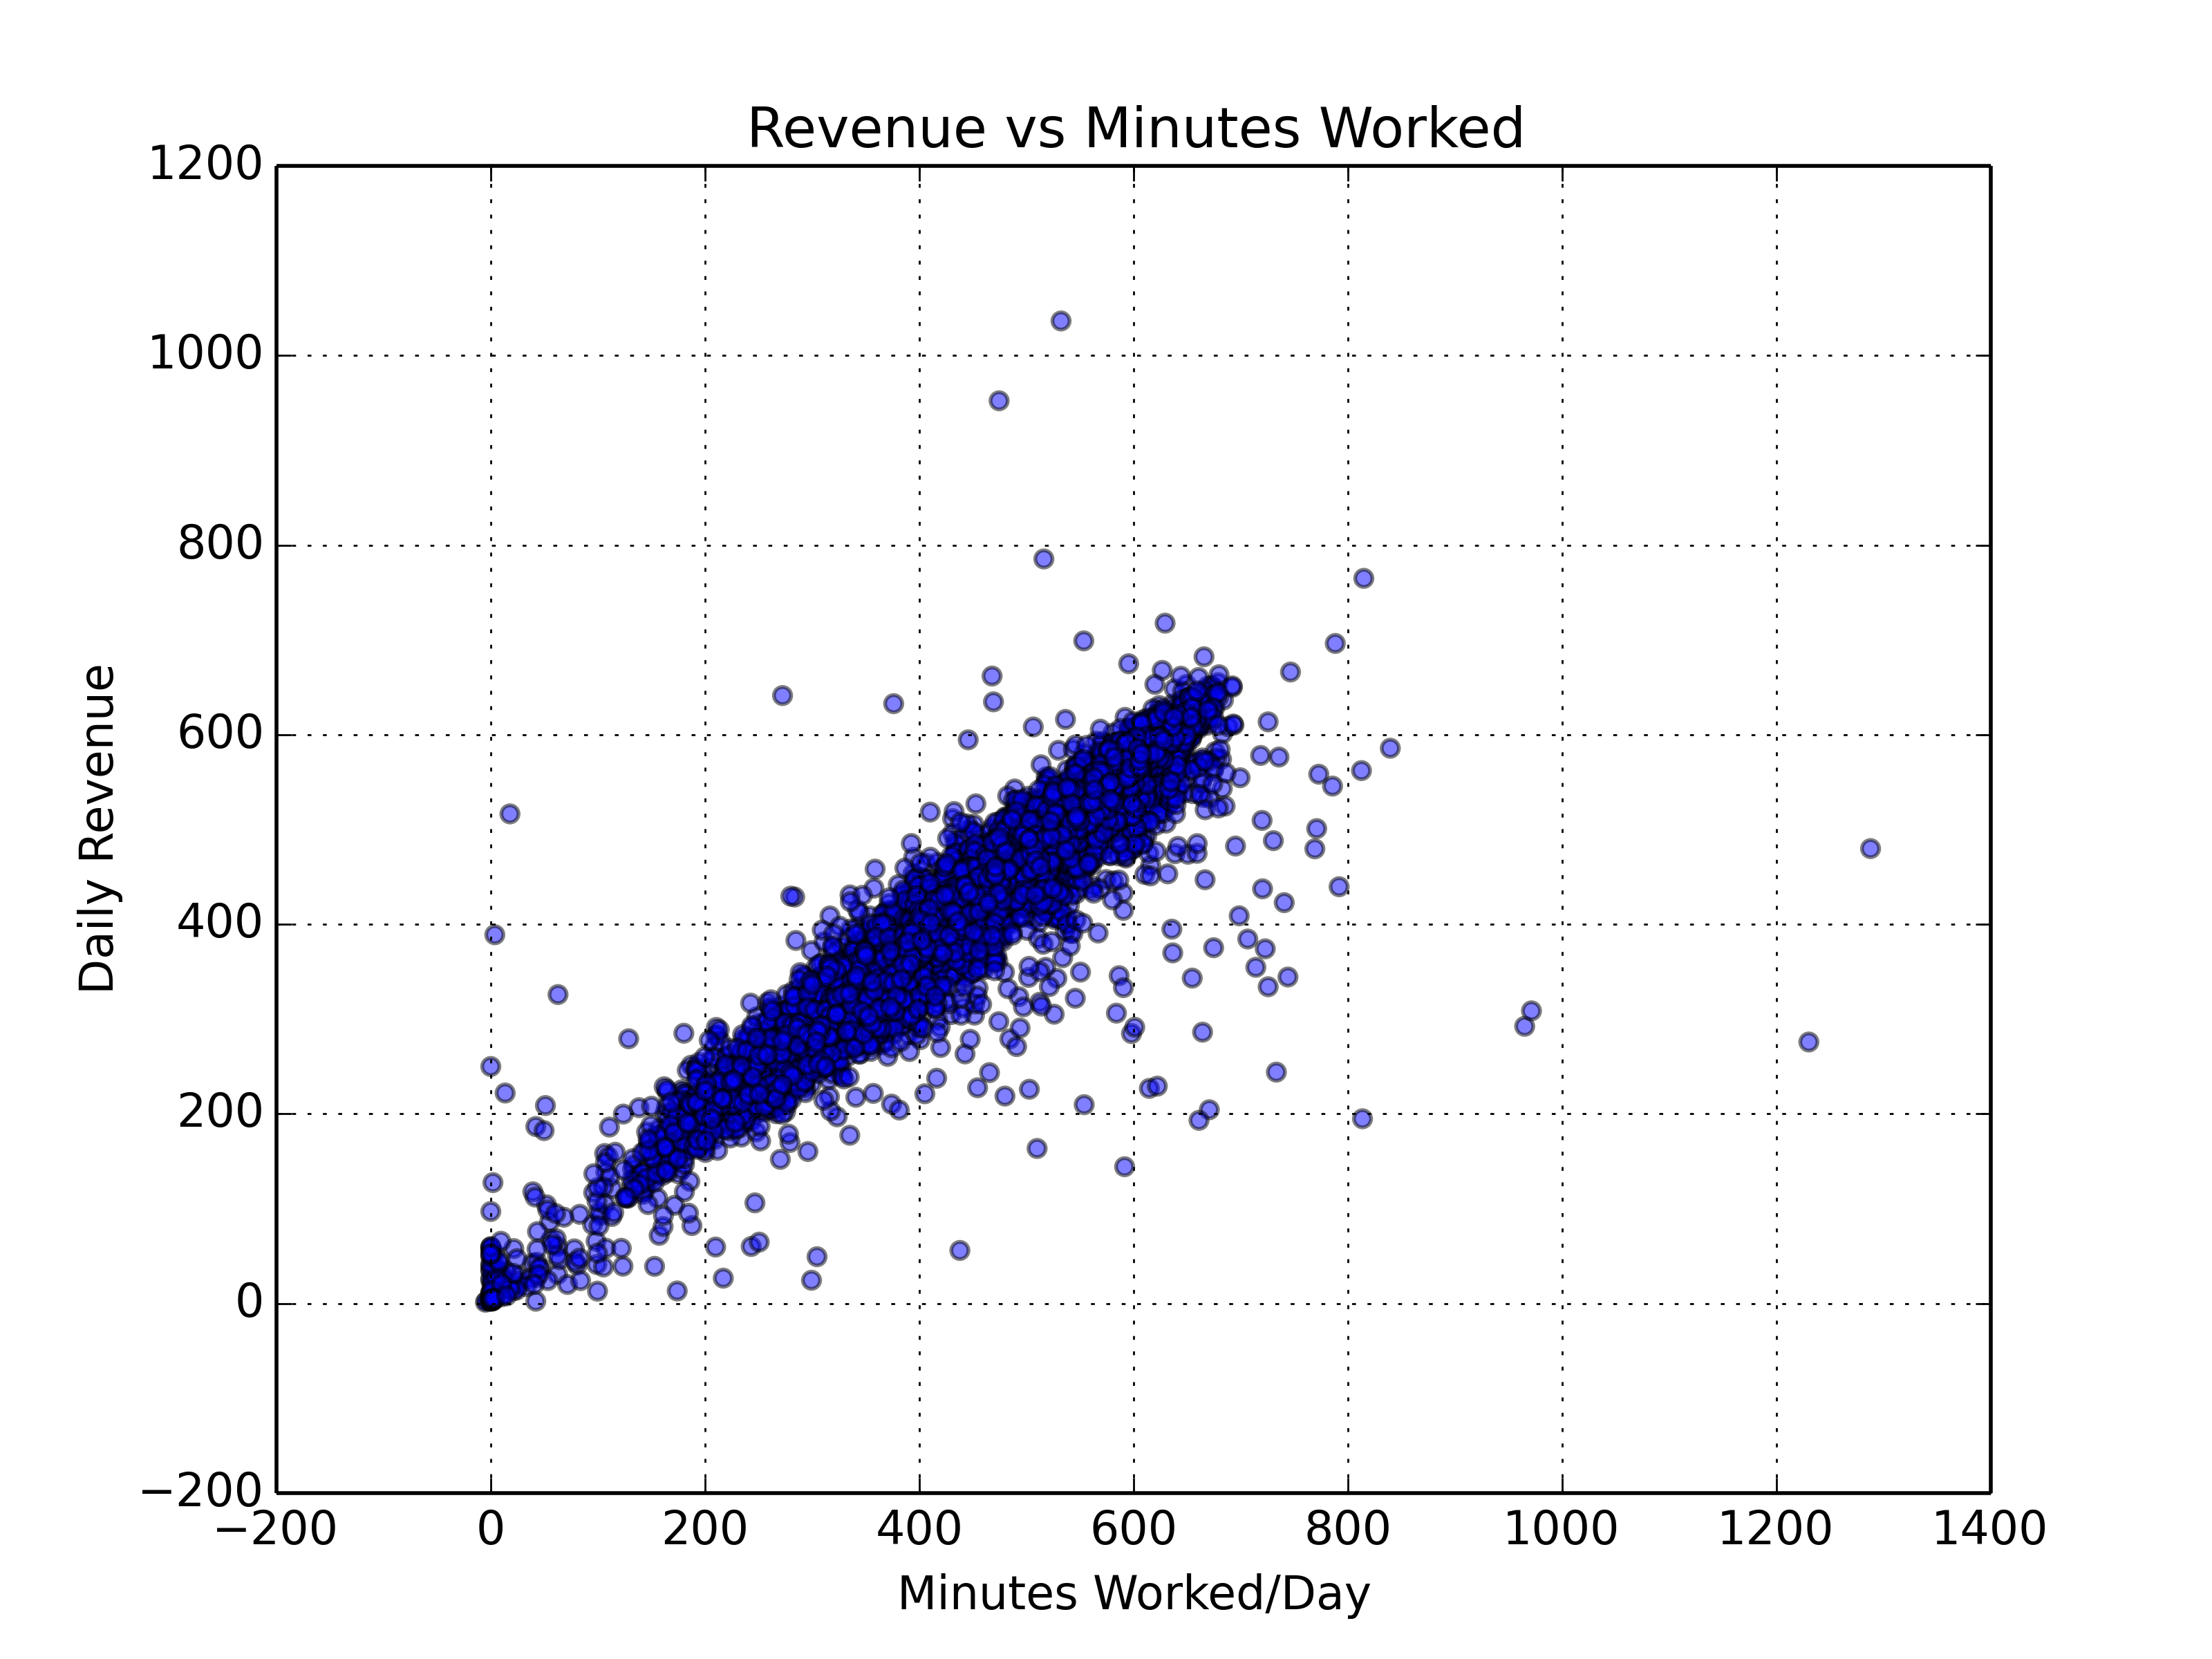
\includegraphics[scale=.35]{Minutes_v_Rev.png}

Though there is nothing surprising about a positive linear relationship between Daily Revenue and Minutes Worked per day, we find the outliers to be interesting. There seems to be a larger spread of outliers below the line than above. However, analyzing the outliers above the line, some seem to work very few minutes an contribute a lot to revenue. Perhaps these drivers are not properly incentivized. It would appear they have much downtime during the day. 

\section{Investigating Question 2: Fare Sensitivities}

\subsection{Experimental Setup}

We leveraged Spark to perform this analysis. Specifically, we performed a number of regressions on the taxi data from 2010 and 2013 (as well as the combined dataset). We set up a regression model of the form:


\begin{multline*}
\text{Fare}[i] = \alpha + \\
	\beta \cdot [\text{distance}[i], \{H[i]\}, \{D[i]\}, \{M[i]\},\{HD[i]\}] +\\
	 \epsilon[i]
\end{multline*}

\noindent with an appropriate number of dummies for the hour of the day, day of the week, month, and hour-day interactions. 

We first made the non binary features standard normal. We then used Spark to fit this linear model. Spark forms the Mean-Squared-Error loss function and performs stochastic gradient descent updates over the inputs to adjust the weights to minimize the function. We utilized 4 m3.2xlarge machines to perform the analysis on AWS. This took about 40 hours (using 100 iterations for each fitting of the model). We then saved the predictions, actual values, and trip datapoint characteristics as a new dataset. 

Additionally, we approximated the variance of $\hat{\beta}$. We found this to be an interesting problem as an exact result would require quadratic time, while an approximate one, like jackknifing would also be too computationally intensive (and of the same complexity though not assuming a functional form like homoskedasticity).  We devised an approximation by randomly sampling 300,000 points (call this $\tilde{X}$) without replacement from our dataset. We then approximated $Var(\hat{\beta})$ by $\text{MSE}*(\frac{N}{300000}\tilde{X}^T\tilde{X})^{-1}$. We used Spark for this sampling procedure to produce our homoskedastic standard errors. 

In order to test time invariance we fit regressions on both the 2010 and 2013 joined taxi data (separately and together). Using Spark, we jointly test whether the regression coefficients are the same as well as perform a test per coefficient for equality. 

The first analysis is conducted via a Chow Test.  The null hypothesis of the Chow Test is that $\beta_{2010} = \beta_{2013}$.  The Chow Statistic is formed by 

$$\frac{(SSR_{comb} - (SSR_{2010} + SSR_{2013}))/k}{(SSR_{2010} + SSR_{2013})/(N_{2010} + N_{2013}-2k)}$$

\noindent which is distributed $F(k, N_{2010} + N_{2013}-2k)$. 

We used Spark to calculate the Sum-of-Squared-Residual terms from the fitted models as well as the counts. This was included in the original regression code (so as to avoid loading the data twice). 

Secondly, we performed a Z-Test on each individual coefficient. Here

$$ Z_i = \frac{\beta_{2010}[i] - \beta_{2013}[i]}{\sqrt(SE(\beta_{2010}[i]) + SE(\beta_{2013}[i]))}.$$
\subsection{Results}

The top 10 most positive $\hat{\beta}$ values are presented in a table below. 

\begin{tabular}{ |l|l| }
  \hline
  \multicolumn{2}{|c|}{10 Largest Positive} \\
  \hline
Distance &	5.50 \\
 Month\_8  &	0.27\\
 hour\_15 &	0.16\\
 hour\_4 &	0.15\\
 hour\_14 &	0.15\\
 hour\_5 &	0.14\\
 hour\_0 &	0.14\\
 Thur &	0.11\\
 Month\_9 &	0.11\\
 Sat\_hour\_23 & 	0.09\\
  \hline
\end{tabular}

The top 10 most negative $\hat{\beta}$ values are presented in a table below. \\

\begin{tabular}{ |l|l| }
  \hline
  \multicolumn{2}{|c|}{10 Smallest Negative} \\
  \hline
 Month\_0 &	-0.34\\
 hour\_7 &	-0.31\\
 Month\_1 &	-0.23\\
 hour\_6 & 	-0.21\\
 Month\_6 &	-0.17\\
 hour\_20 &	-0.16\\
 hour\_19 &	-0.16\\
 Mon &	-0.14\\
 hour\_10 &	-0.13\\
 Month\_3 &	-0.12\\
  \hline
\end{tabular}\\


The dummies all had very high standard errors while distance was highly significant. We suspect that the dummy standard errors would be lower without our approximation.  Please see outputs for exact betas and standard errors.

We find the above results interesting in terms of driver incentives. Those who work part-time should be partial to working time periods that align with high dummy values (these would lead to higher fares and tips for conceivably the same distances). They should avoid the low beta value periods. If the taxi company wants to smooth availability, assuming drivers already have some idea about these results, they should offer financial incentives by time period to even out the beta distribution. 

The Chow Test yielded that we cannot reject the null hypothesis that the sensitivities are jointly equal for the 2 different years. However, the distance beta Z-value would lead us to reject the hypothesis of equality for the sensitivity for the two different years. The other Z-values are not significant. Hence, the results of the Z-test and Chow test seem consistent. 


\section{Investigating Question 3: Driver Performance v Fare Sensitivities}
Based on the regression output from the previous section, we plot the residual (i.e. actual fare minus predicted fare) for each trip and bin them into histograms.  
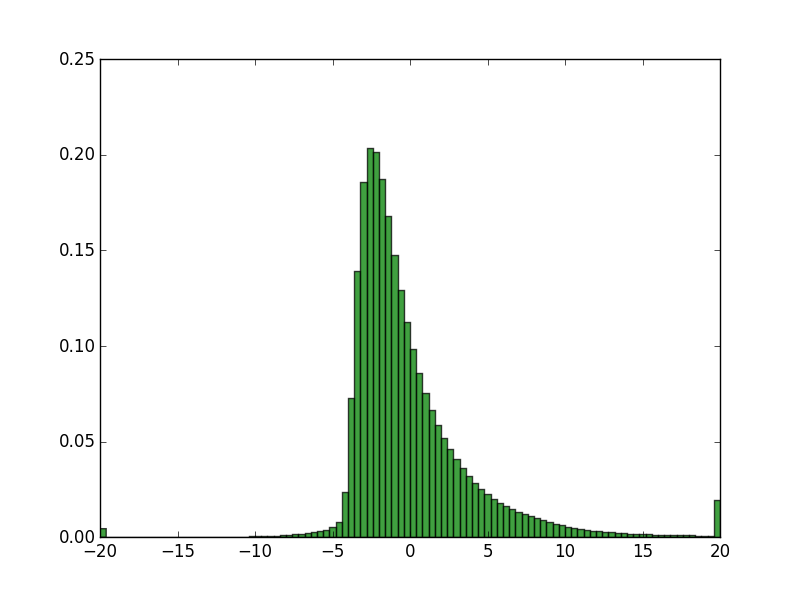
\includegraphics[scale=.35]{figure_1.png}
While much the error may be coming from the fact that our regression model is very simple (for example, it doesn't take into account the fact that a distance of 1 mile means very different things in midtown versus in suburbs of Queens), there does seem to be a cohort of trips in which the customer is overcharged. \\
Next we investigate whether customers who are overcharged (i.e. have high residuals) give less tip. Below is a scatter plot of residuals (x-axis) versus tip percentage (y-axis). While the relationship is far from clear, there does seem to be a slight negative relationship between tip percentage and residual.
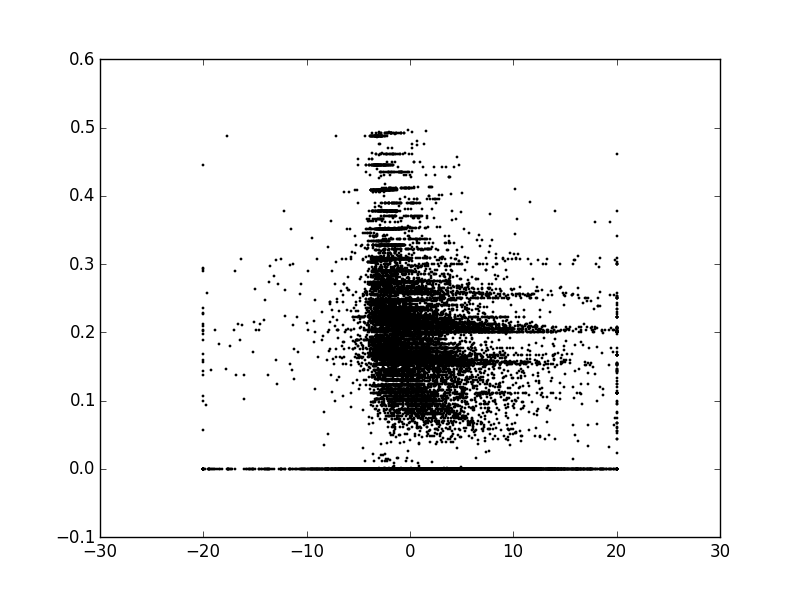
\includegraphics[scale=.35]{figure_2.png}

\section{Investigating Question 4: Previous Earnings v Behavior}
\subsection{Experimental Setup}
For this analysis, we return to MrJob. Here our map task outputs $\text{[driver, (pickup day, tip percentage)]}$
for every entry in our joined taxi data. We then implement a rather complicated reducer.  For every driver, the reducer computes the tip percentage median per day. This is used to control for possible trends in the data (we assume a day is small enough to not contain an economic trend). We then iterate through all of the tip percentages each day and count the number of times a tip above the daily median is followed by another vs one below the daily median. These are `above-above' vs `above-below'. By definition, half the tips must be above the median and half below. Hence, we find the frequency of `above-above' vs `above-below' to be a good test for a behavioral factor. For each driver we output the tip statistic

$$\frac{Count(`above-above')}{Count(`above-above') + Count(`above-below')}.$$

We then aggregate these results and look at the distribution over drivers. The running time and experimental setup is nearly identical to our the MR jobs. 
\subsection{Results}
The resulting distribution is depicted below. 
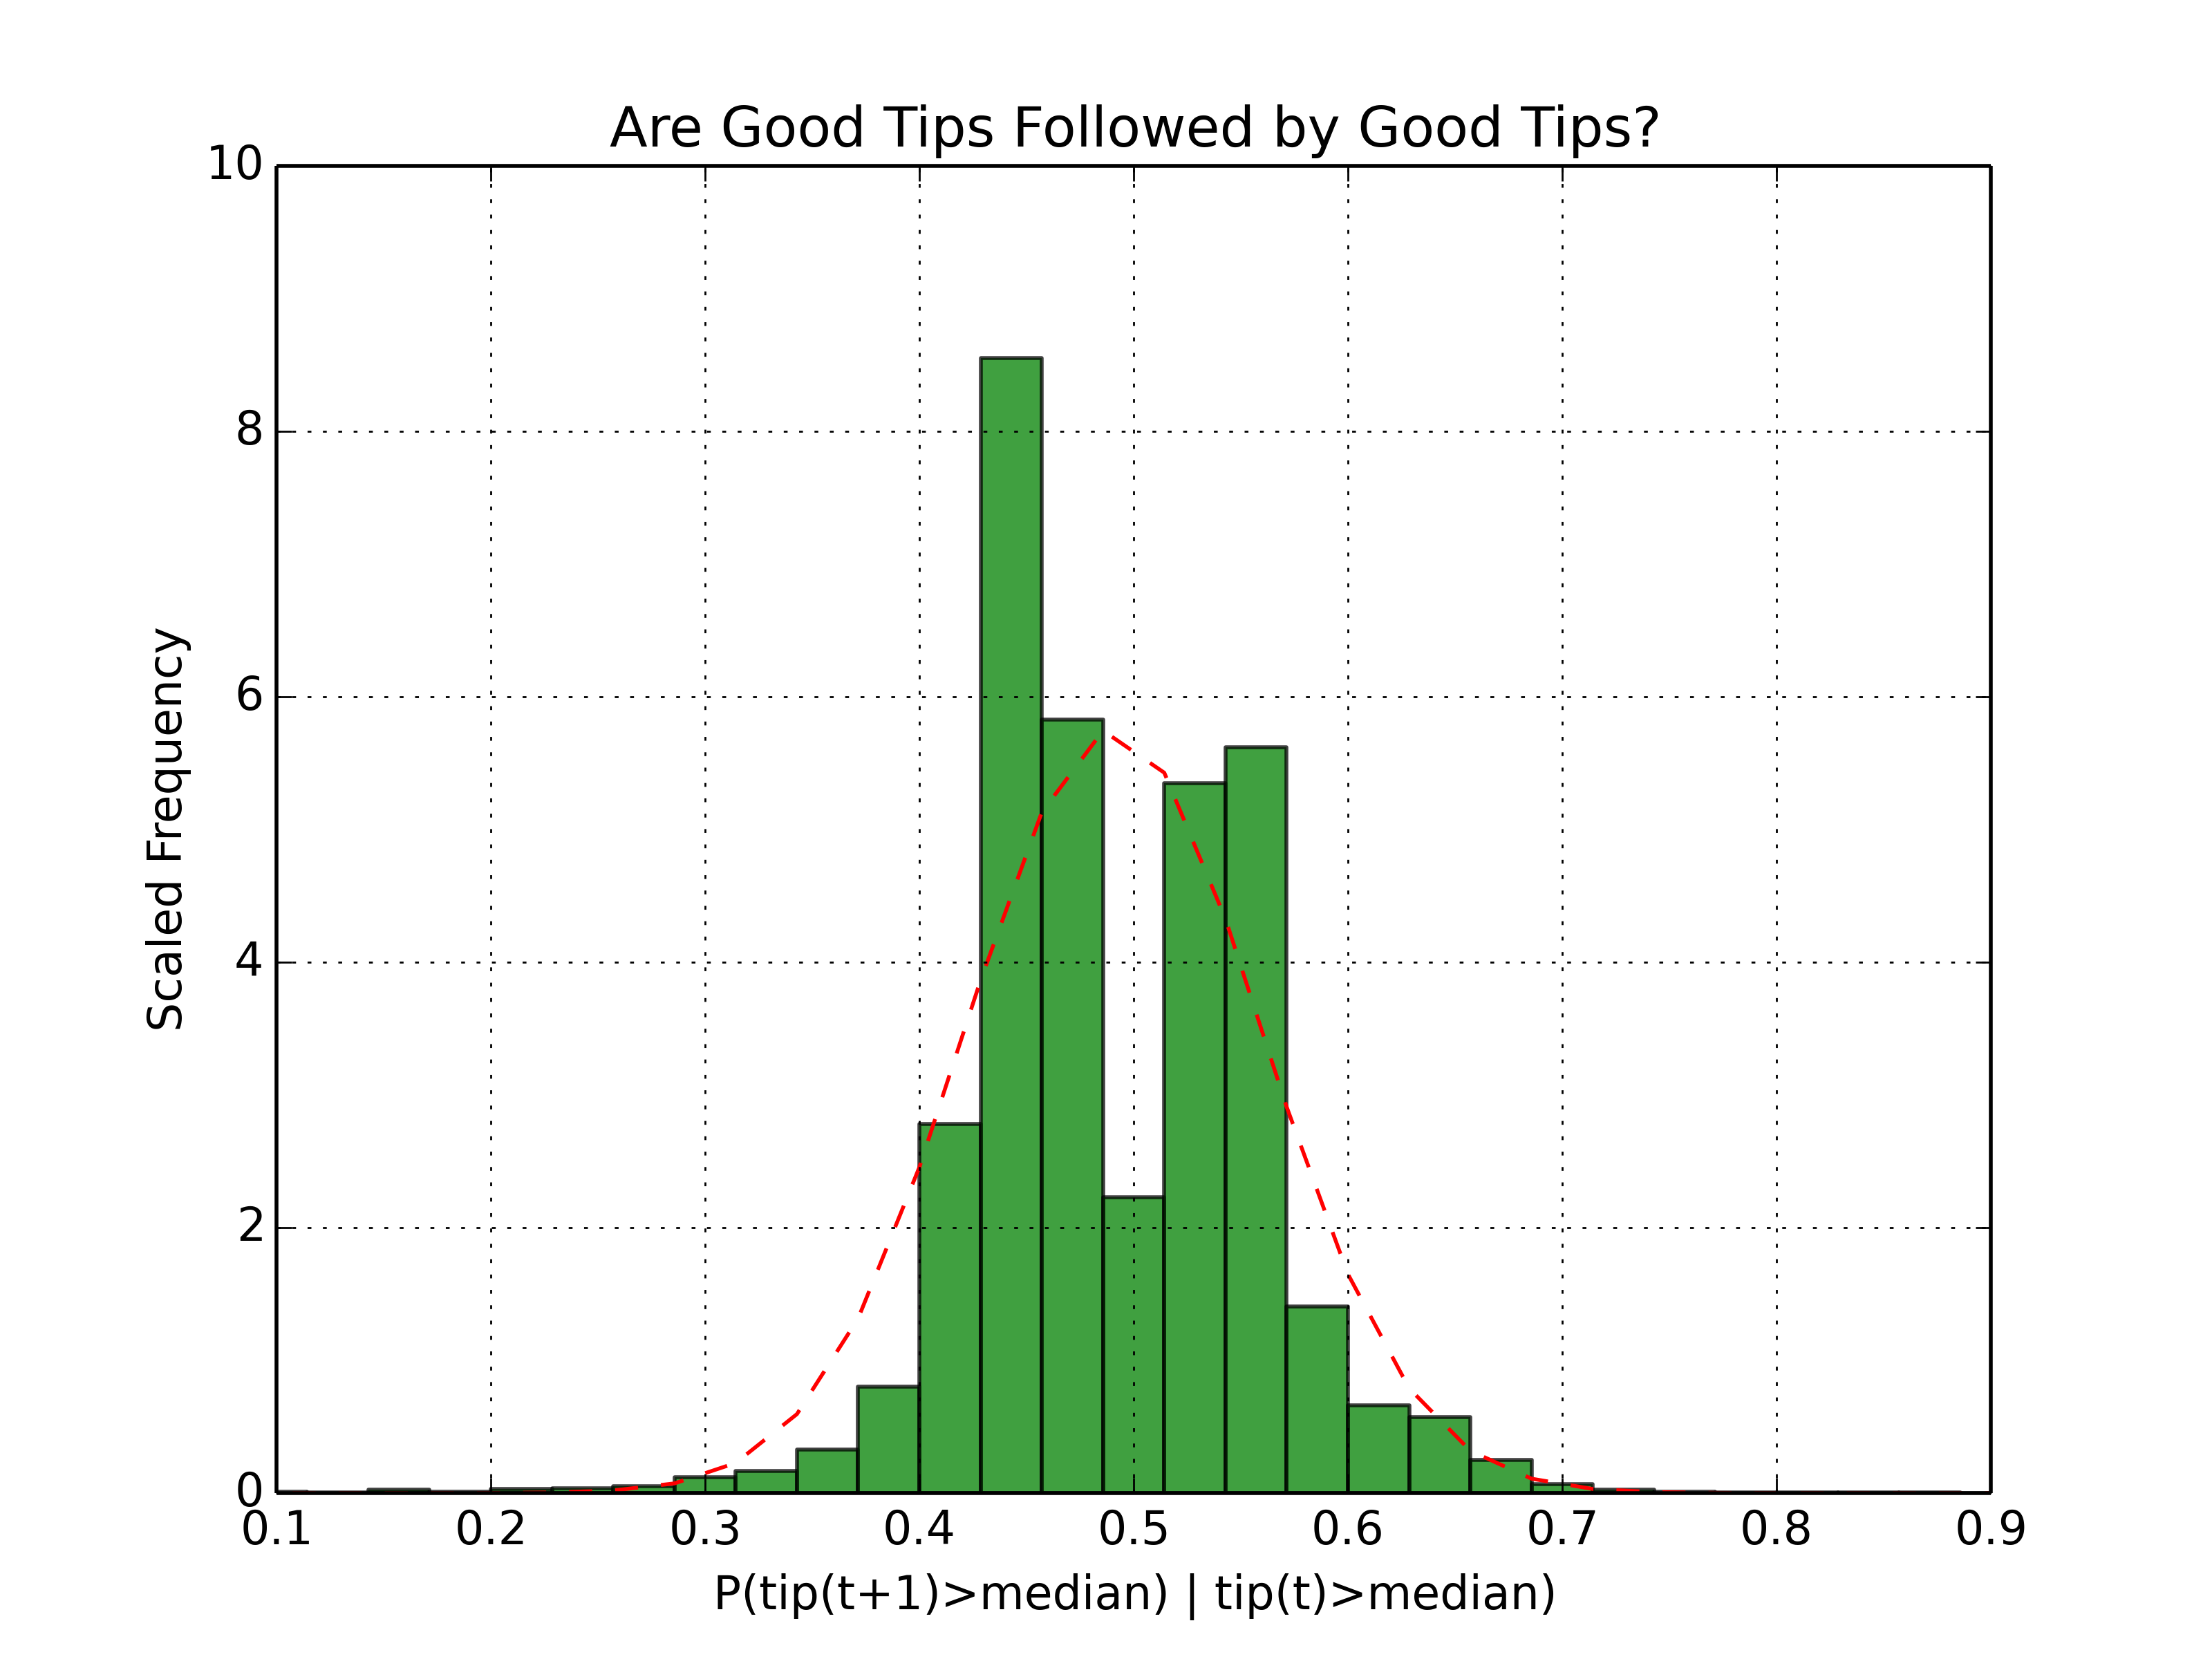
\includegraphics[scale=.35]{hothand.png}

For various bin sizes, we find a similarly bimodal result. The red line represents the resulting normal distribution given our input data. Here, we see that the distribution is definitely not normal. However, behavior is on both ends of the spectrum. Moreover, we are unsure if it is exactly the behavior we thought we were measuring in the first place. We assumed that a good tip would improve driver moral and lead him to try harder on the next trip.  Then he would be more likely to get a larger tip.  Here we also see that for many drivers a good tip is more likely followed by a bad tip.  Either a good tip leads to laziness or we need more controls. Perhaps a time-of-day control could improve the experiment assuming that tipping trends change in morning vs afternoon vs night. This may be a reasonable assumption. We did not have sufficient funds to continue this analysis on AWS. 

\section{Investigating Question 5: Average Tip Percentage vs Income}
Next, we look at whether there is a relationship between passenger income and tip percentage. This involves several steps.
\begin{itemize}
\item We first create a grid of zip codes from querying latitude and longtitude for NY area based on Python's \texttt{geopy} package.
\item Then we use the grid to match dropoff lat-long to zip code via MapReduce. Note that because the matrix is created already, zip code lookup on the grid take $O(1)$ time.
\item We make the (crude) assumption that people who are getting dropped off are going home. We use the census data to match the zip code to median household income.
\item We calculate the average tip percentage for that zip code to investigate the relationship between median household income for dropoff zip code and average tip percentage.
\end{itemize}

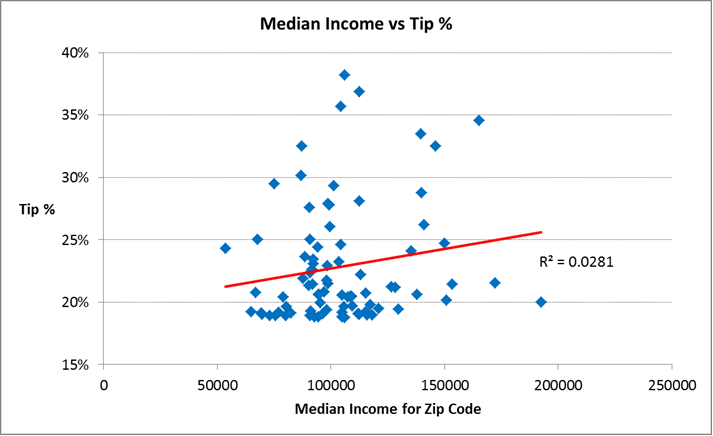
\includegraphics[scale=.4]{zip_income.png}
As can be seen from the above chart, there seems to be a very small positive relationship between median household income and average tip percentage.
%------------------------------------------------

\section{Concluding Remarks}

We have outlined a number of factors that affect driver behavior. Moreover, we provide a guide on how to use modern big data tools for this type of analysis. Each question could be greatly expanded into more parts. We offer this report as a basic framework to aid in such a further investigation. 





%----------------------------------------------------------------------------------------

\section{Appendices}

\subsection{Running the Code}

Our code is available at \\

\noindent https://github.com/ssz225/bigdata\_final.\\

\noindent Each component has a corresponding question folder with instructions as to how to run the code. We have excluded all of our AWS access information from the code and put in dummy values.  The joined input data is available at \\

\noindent https://s3.amazonaws.com/trip-fare-join/2010/part-0000X\\
\noindent https://s3.amazonaws.com/trip-fare-join/2013/part-0000X
\\\\\
where X ranges from 0 to 6.

\subsection{Individual Contributions}
\subsubsection*{Daniel}
\begin{itemize}
  \item Preprocessing Taxi Data Inputs
  \item Question 1: Driver Productivity Differences
  \item Question 2: Fare Sensitivities
  \item Question 4: Previous Earnings v Behavior
  \item Report - Writing
  \item Code - Organization for Submission
\end{itemize}


\subsubsection*{Yoon}
\begin{itemize}
  \item Question 3: Driver Performance v Fare Sensitivities
  \item Question 5: Average Tip Percentage vs Income
  \item Presentation - Writing and Formatting
  \item Report - Writing
  \item Code - Organization for Submission
\end{itemize}


\end{multicols}

\end{document}
